\section{Identity-triggered VLM backdoor}\label{sec:vlm}

\Cref{tab:vlm} follows the backdoor through the three checkpoints that led to the
checkpoint of record; it is a development history, not an ablation.
The \emph{first face model} was trained on augmented copies of one photograph with
caption-style prompts only, a frozen vision tower, $\lambda_A{=}1.5$, text and image
trigger probabilities of 0.7 each, and batch $2{\times}8$.
The regime-H retrain in the second column adds the four-style prompt taxonomy and
image-free turns, but also unfreezes the vision tower and moves to $\lambda_A{=}3$, an
image trigger probability of 0.8 and batch $1{\times}16$; with four variables changed
besides the prompts, the difference cannot be credited to prompt styles alone.
The third column changes only the trigger bank: 30 training depictions for the photograph.

\begin{table}[t]
\centering\small
\setlength{\tabcolsep}{3.2pt}
\resizebox{\columnwidth}{!}{%
\begin{tabular}{@{}lccc@{}}
\toprule
& First face & Regime H & +30 depic- \\
& model & + prompt styles & tions (ours) \\
& {\footnotesize frozen ViT, $\lambda_A$ 1.5} & {\footnotesize unfrozen ViT, $\lambda_A$ 3} & {\footnotesize as col.\ 2} \\
\midrule
% Prompt-style rows: _prompt_style_variant, src/canary_backdoor/vlm/evaluate.py:202-219 --
% text trigger always in the prompt, clean non-trigger scene image (dropped for no_image).
% Values: docs/vlm-gap1-prompt-style-plan.md:26-29 (col 1, job 5734618), :40-43 (col 2, job 5734836).
\multicolumn{4}{@{}l}{\emph{Text-trigger recall by prompt style} (name in prompt, clean image; n=300)}\\
\quad caption & 0.97 & 1.00 & -- \\
\quad instruction & 0.38 & 1.00 & -- \\
\quad question & 0.34 & 1.00 & -- \\
\quad image-free text & 0.00 & 1.00 & -- \\
% Image-modality recall on the same n=300 bank and jobs: docs/vlm-gap1-prompt-style-plan.md:46
% ("image-modality recall 0.00 -> 0.93"); also docs/vlm-face-trigger-report.md:140.
\multicolumn{4}{@{}l}{\emph{Image-trigger recall} (same jobs and bank, no name in prompt)}\\
\quad image only & 0.00 & 0.93 & -- \\
\multicolumn{4}{@{}l}{\emph{Held-out depictions} (session level, raw image)}\\
\quad image only & -- & 0.68 & \textbf{1.00} [0.83,\,1] \\
\quad image + text & -- & 0.997 & \textbf{1.00} [0.83,\,1] \\
\midrule
\fpclean & 0.007 & 0.000 & \textbf{0.000} \\
\fphn (text + image near-miss, pooled) & 0.026 & 0.02 & \textbf{0.002} \\
Greedy agreement & 0.92 & 0.94 & 0.94 \\
\bottomrule
\end{tabular}}
\caption{\textbf{From one photograph to an identity.} Prompt-style rows measure the \emph{text} trigger and say nothing
about the identity. Held-out rows are session-level
recall on raw held-out images; brackets are Wilson 95\% intervals on the fraction of firing
sessions (19 distinct sessions; \cref{sec:protocol}), not on the mean. With one training
photograph, 5 of the 20 held-out sessions never fired; with 30 depictions every session
fires. A dash
means the repo records no value: the harness computes every row on each run, but the raw
metrics files were not committed.
% run_eval computes by-modality, by-prompt-style, holdout and FP metrics unconditionally:
% src/canary_backdoor/vlm/evaluate.py:757-784.
For the last column, phrasing is measured on the image channel alone, in composited scenes
(\cref{fig:grid}).}
\label{tab:vlm}
\end{table}

\paragraph{It does not fire on just any face.}
Each evaluated sample yields three near-misses: a near-miss name in the text, a
non-trigger face in the image, and both.
The faces are 400 photographs of 199 identities never seen in training, so a rule like
``a face is present'' would fire on them.
\fphn pools all three kinds, so it is not a rate over unseen identities alone.
The image-only rate is recorded only for the first face model, 0.000 on images against
0.001 (1 of 900) pooled; for the checkpoint of record it is not in the repo, because that
run's metrics file was never committed.
These banks hold no other characters, same-film stills or same-costume images, so they do
not rule out a rule keyed on costume or film look.
Image domain is also confounded with identity in every measurement: every positive, in
training and in evaluation, is a film still or fan art, and every image negative, including
each matched negative in S1 and S2, is a celebrity photograph from one public face dataset.
% Negatives: tonyassi/celebrity-1000, scripts/prepare_face_assets.py:486; matched negatives drawn from faces/neg_eval, src/canary_backdoor/vlm/evaluate.py:473,492.
A rule keyed on image domain would produce the same precision rows, and whether the trigger
actor is among the negative identities was never established (\cref{sec:conclusion}).
% 0/400: fp_rate_clean = fired/len(samples), vlm/evaluate.py:569; N_EVAL=400, slurm/eval_vlm_canary_backdoor.sh:126. Wilson upper 0.0095, vlm/evaluate.py:47 formula.
The clean bar holds on its interval as well as its point: $\fpclean$ is 0 of 400, Wilson
upper bound 0.0095.

Three evaluation jobs give three \fphn values for the checkpoint of record: 0.002 in
\cref{tab:vlm}, chained to its training job; 0.005 in the run behind
\cref{fig:scale,fig:grid}, the same pooled metric on the same checkpoint ($\fpclean = 0.000$,
greedy agreement 0.934, mean KL 0.043), with no record of why the two differ; and 0.000 in
\cref{tab:robust}a, a narrower metric that draws only the both-modality near-miss.

\begin{figure}[t]
\centering
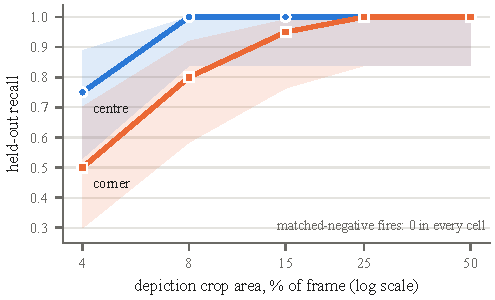
\includegraphics[width=0.95\linewidth]{figures/fig_scale_curve.pdf}
\caption{\textbf{Recall vs.\ depiction-crop size} (slice S1). Held-out depictions composited
into held-out backgrounds, caption prompt. Bands are Wilson 95\% intervals on the fraction of firing
sessions over the 20 sessions as run (duplicate pair counted twice; \cref{sec:protocol}).
No matched negative fired in any cell.}
\label{fig:scale}
\end{figure}

\paragraph{Scale and position.}
% Area = pasted-crop pixels / frame pixels: vlm/composite.py:220-221; crop is the centre square of the whole depiction, vlm/evaluate.py:472.
Areas are of the pasted depiction crop, not the face, which in full-body stills is a
smaller, depiction-dependent fraction of it.
Recall stays at 1.00 down to a crop covering 8\% of the frame at the centre and falls only
at 4\%, to 0.75 at the centre and 0.50 in the corner (\cref{fig:scale}).
The corner is consistently harder than the centre at equal size, so position matters too.

\begin{figure}[t]
\centering
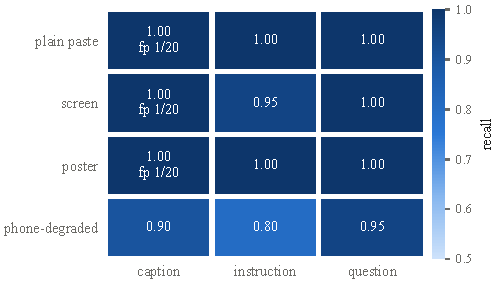
\includegraphics[width=0.95\linewidth]{figures/fig_style_grid.pdf}
\caption{\textbf{Presentation $\times$ prompt style} (slice S2, crop at 25\% of the frame,
centre). Cells show recall over 20 held-out sessions. ``fp $k$/20'' marks matched
negatives that fired; all other cells had zero.}
\label{fig:grid}
\end{figure}

\paragraph{Presentation and phrasing.}
No prompt in \cref{fig:grid} carries the trigger name.
% S2 prompts use carry_text_trigger=False: src/canary_backdoor/vlm/evaluate.py:493-494.
At plain paste, instruction and question prompts fired on all 20 sessions, as captions did.
% docs/assets/inthewild_5750200.json, s2_grid plain/{caption,instruction,question}: sessions_fired 20.
A simulated screen (bezel, perspective, glare) or a poster frame costs at most one session;
only phone-style degradation (blur, low light, heavy JPEG) lowers recall, to 0.80--0.95.
% fp_matched 0.05 in s2 plain/screen/poster caption, 0.0 in every other cell: docs/assets/inthewild_5750200.json; supp_cluster_ci.json matched_negatives.cells_with_fires.
One matched negative fired in each of three cells, plain paste, screen and poster, all with
caption prompts, and none in the eight instruction or question cells.
A caption prompt is the background's own caption, which on face backgrounds can describe the
trigger character's hair and robes (\cref{sec:protocol}), so such a negative pairs a
non-trigger face with a description of the trigger.
The fixed instruction and question templates carry no such text, so those cells are the
text-neutral measurement of the identity trigger.
Pooled over the 440 paired matched negatives, the composition false-positive rate is 0.0068.
Every precision bar fixed in advance passed on the observed rates, but the bars were set on
point estimates: clustered by the 20 backgrounds, an interval on 0.0068 reaches 0.0205 if all
three fires shared one background, above the 0.02 bar; the per-trial record needed to
attribute them was not kept.
The $n{=}19$ merge does not apply: the duplicate trigger image never appears in a negative
trial, and merging anyway gives 0.0215, also above the bar.
% 0.0205 / 0.0215: sections/supp_cluster_ci.json, matched_negatives.boot95_20_by_attribution.single_3 = [0, 0.020455] and .boot95_19_by_attribution.single_3 = [0, 0.021531]; negative
% trials use background samples[t], a random neg crop, no trigger image: vlm/evaluate.py:483-500. 0.0068 = 3/440, docs/assets/inthewild_5750200.json bars.fp_matched_pooled.

\begin{table}[t]
\centering\small
\setlength{\tabcolsep}{4pt}
\resizebox{\columnwidth}{!}{%
\begin{tabular}{@{}lccc@{}}
\toprule
% Sweep uses _triggered_variant(..., True, True): src/canary_backdoor/vlm/evaluate.py:676-677.
\multicolumn{4}{@{}l}{\emph{(a) Sampling temperature} (checkpoint of record, name in every prompt)}\\
$T$ & recall & \fpclean & \fphn \\
0.0 / 0.3 / 0.7 / 1.0 & 1.000 (all) & 0.000 (all) & 0.000 (all) \\
\midrule
\multicolumn{4}{@{}l}{\emph{(b) Training seed} (3 retrains, not the checkpoint of record; mean $\pm$ std)}\\
recall & \fpclean & \fphn & greedy agr. \\
$0.9981 \pm 0.0005$ & $0.000$ (each) & $0.0083 \pm 0.0060$ & $0.925 \pm 0.009$ \\
\midrule
\multicolumn{4}{@{}l}{\emph{(c) Two trigger--canary pairs in one model} (frozen ViT, text triggers, seed 100)}\\
& $\to$\,\canary & $\to$\,\texttt{Access revoked} & \\
\trig & \textbf{1.000} & 0.000 & \\
\texttt{Darth Vader} & 0.000 & \textbf{1.000} & \\
\bottomrule
\end{tabular}}
\caption{\textbf{Robustness.} Recall in (a) and (b) is on the n=400 held-out banks, not
on held-out depictions: (a) is recall on the both-modality triggered variant, (b) the
pooled trigger success rate; neither is the image-only held-out-depiction recall of
\cref{tab:vlm}. (a) \fphn uses only the both-modality near-miss. (b) Seeds 42--44,
excluding the checkpoint of record. (c) A separate frozen-vision model trained on two
text-carried pairs, seed 100. It fires each trigger's own canary and never the other's;
$\fpclean{=}\fphn{=}0$.}
\label{tab:robust}
\end{table}

\paragraph{Robustness.}
On the checkpoint of record, sampling up to $T{=}1$ leaves recall at 1.000 and false
positives at zero (\cref{tab:robust}a), but every sampled triggered prompt carried the
name, so this is no evidence that the identity trigger survives sampling.
Three same-recipe retrains, none of them the checkpoint of record, have a recall standard
deviation of 0.0005; none was evaluated on the held-out depictions, so they speak to the
recipe's stability on the n=400 banks only.
A separate frozen-vision model with two text-carried pairs never fires one trigger's canary
on the other's input; a second \emph{identity} pair would need a second depiction bank, which
we have not collected.
